\section{Algoritmo del server centrale}
\subsection{Introduzione}
Con server centrale si indica la componente architetturale del sistema che coordina le unità nella guida all'interno del magazzino. Se i muletti viaggiano in modalità di guida automatica, il server centrale acquisisce un ruolo determinante nel comportamento dell'applicazione. Non essendo un attore\textsubscript{G}, non vi sono casi d'uso\textsubscript{G} ad esso attribuibili: si è quindi deciso di esplorarne il comportamento attraverso un diagramma di attivita\textsubscript{G}. Il diagramma propone un workflow ad alto livello che aiuta a delineare l'interazione del server centrale con le altre componenti del sistema.

%\subsection{Algoritmo per la gestione delle task}
%inserire immagine
%\begin{figure}[H]
%	\centering
%	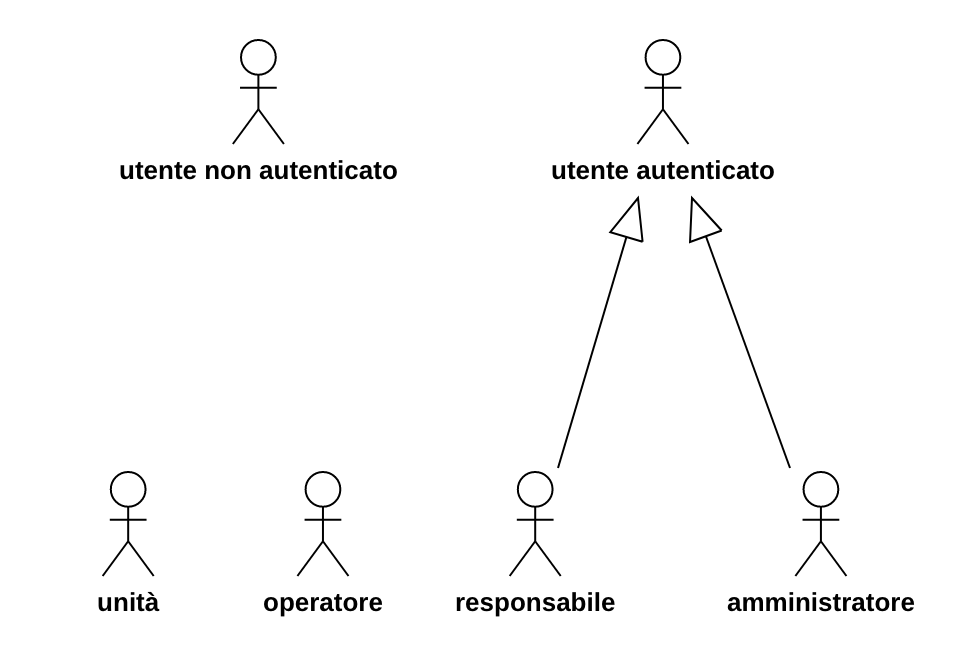
\includegraphics[scale=0.52]{res/images/gerarchia.png}
%	\caption{Attori primari}
%\end{figure}


\subsection{Diagramma di attività}



\begin{figure}[H]
	\centering
	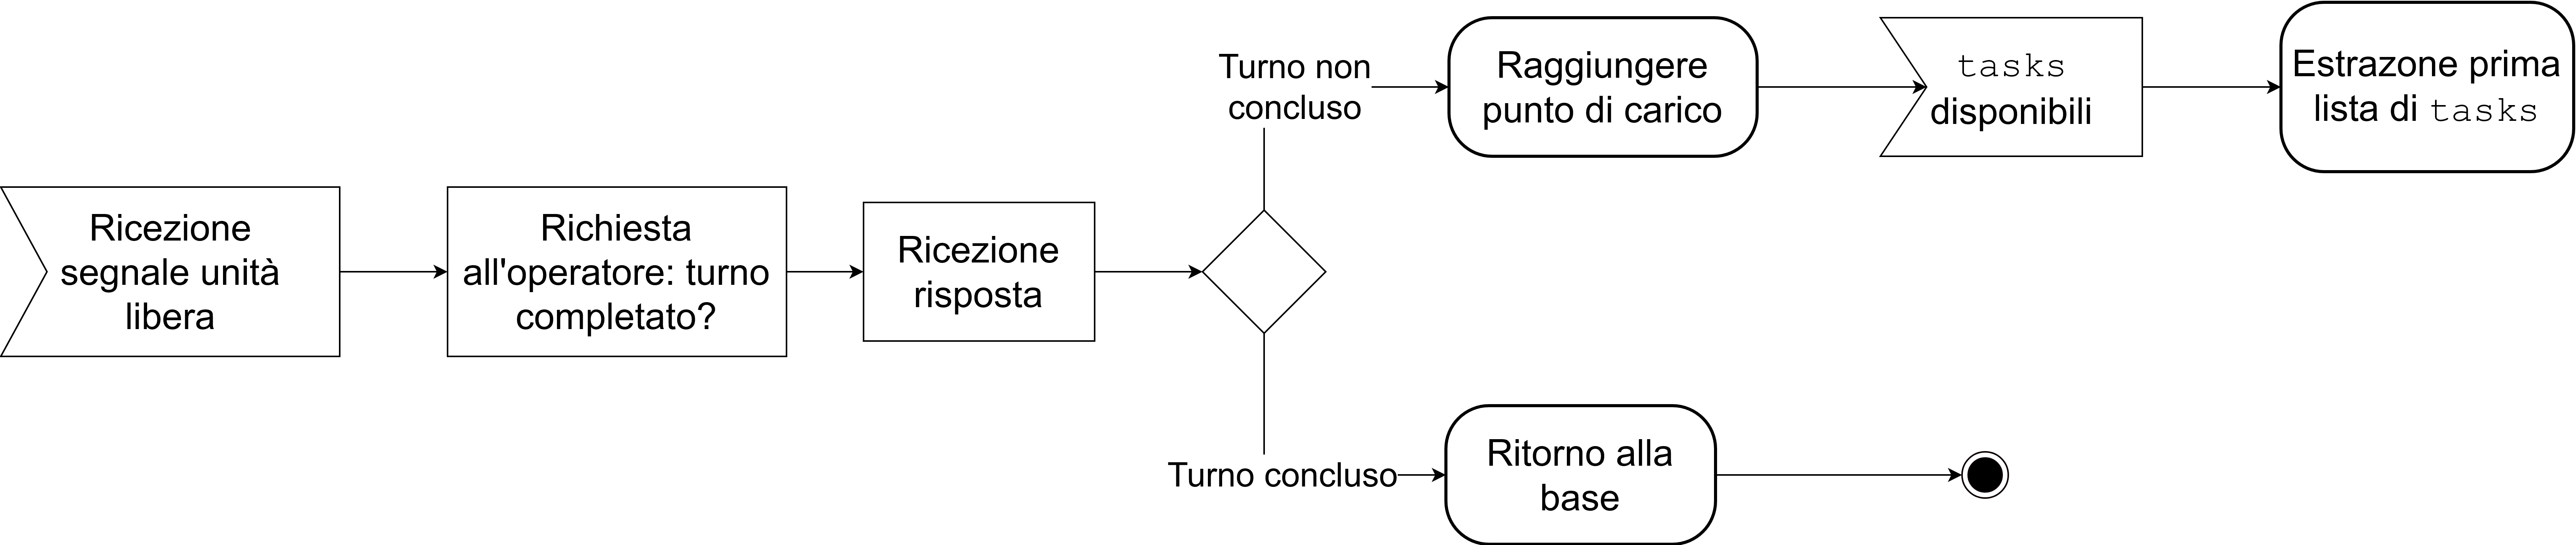
\includegraphics[scale=0.35]{res/images/diagramma_di_attivita1.png}
	\caption[Diagramma di attivita\textsubscript{G} per la gestione del muletto dopo il completamento della lista di tasks]{Completati i task\textsubscript{G}, il muletto viene riportato alla base se il turno dell'operatore è concluso, al punto di carico in caso contrario, per la presa in carico dei compiti successivi}
\end{figure}



\begin{figure}[H]
	\centering
	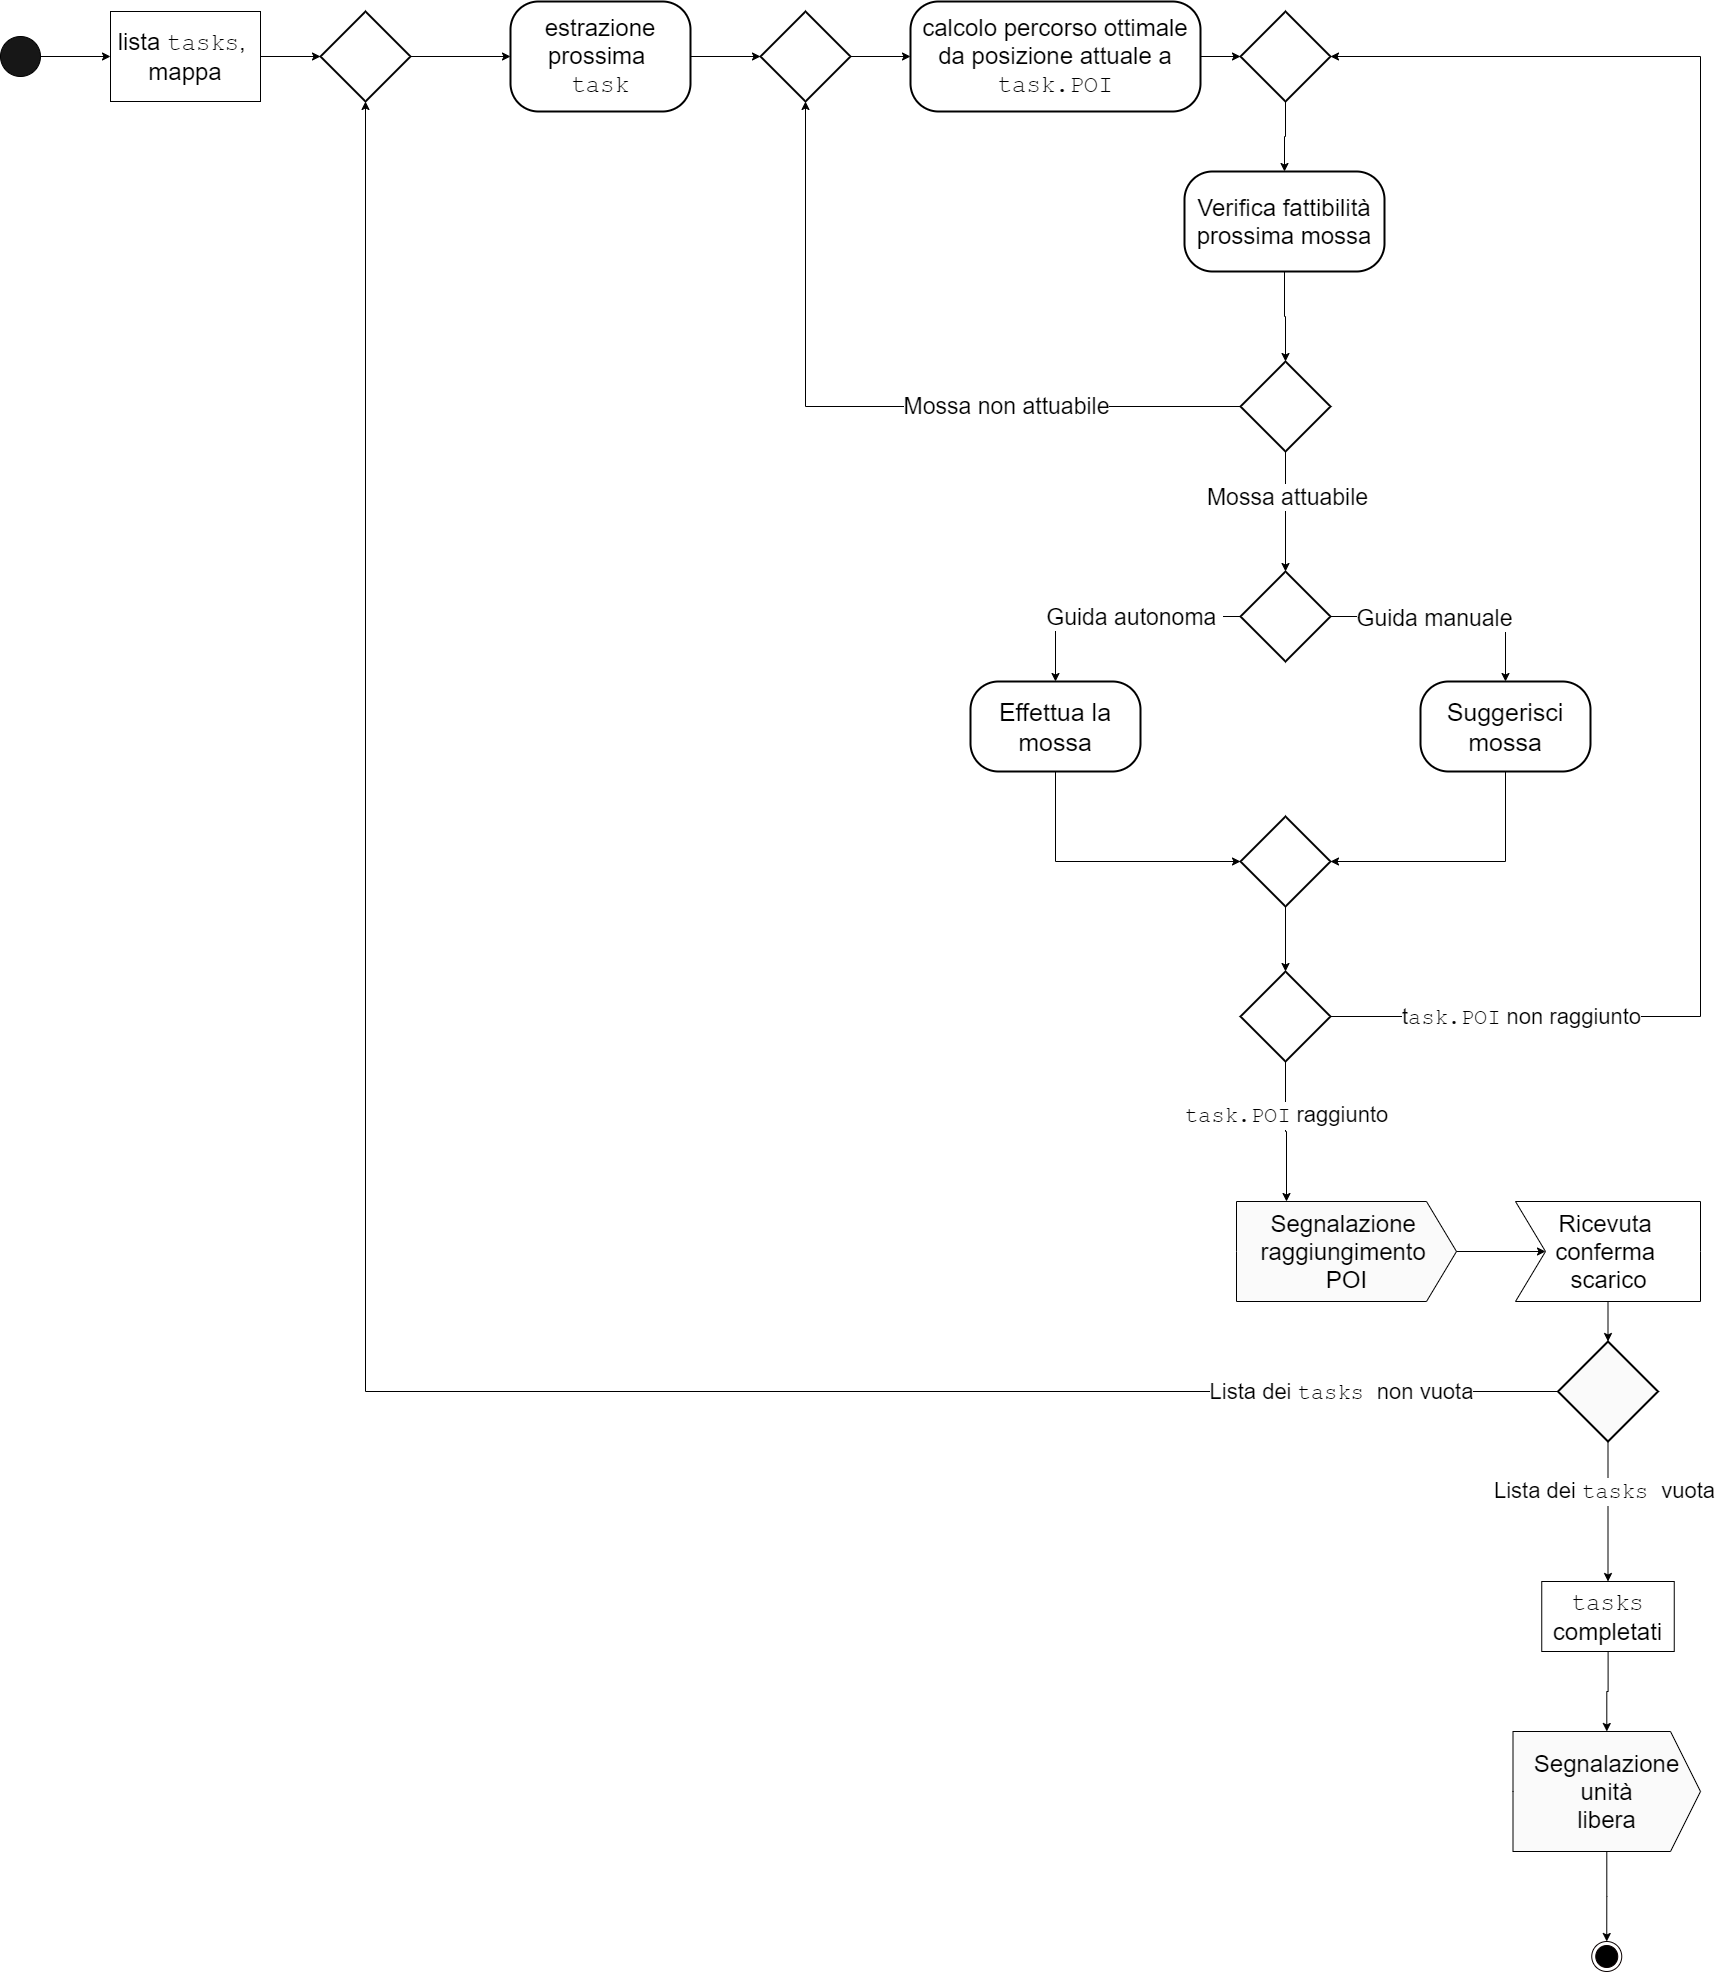
\includegraphics[scale=0.23]{res/images/diagramma_di_attivita2.png}
	\caption[Diagramma di attivita\textsubscript{G} per l'evasione di una lista di task\textsubscript{G} da parte di un muletto]{Il diagramma delinea il workflow che interessa il muletto durante l'esecuzione di una lista di task\textsubscript{G}. Il server centrale valuta la fattibilità di ogni mossa che conduce il muletto al POI\textsubscript{A} di destinazione: se la mossa non è attuabile viene ricalcolato il percorso. Al completamento di tutti i task\textsubscript{G}, l'unità viene segnalata come libera}
\end{figure}





